 % -*- root: ../medieninformatik-arbeit.tex -*-
\documentclass[../medieninformatik-arbeit.tex]{subfiles}
\begin{document}
\label{ch:proto}
\section{Prototype Design}
This chapter presents the process of developing the designs for the activity sculpture and the web configurator. In the first section the requirements for the activity sculpture are presented and four different designs that attempt to fulfill the requirements are presented. Finally the validation process for the sculpture to be designed will be discussed. The second section is devoted to the design process of the customization system. This comprehends not only the user interface but also the user experience while operating the system. After a process where three different concepts were ideated, through the validation of the design the final prototype is chosen. 

\subsection{Activity Sculpture Design}
The activity sculpture and the configurator are strongly interconnected as depending on the design, the sculpture will influence the quantity of controls to be taken into consideration for the design of the configurator giving users greater or lesser freedom for manipulating the the sculpture. As we discussed in section \ref{sec:activitysculptures}, activity sculptures portray different attributes inherit from their physical nature. This why a different approach for designing physical data visualizations is needed. For this purpose the design taxonomy proposed by Vande Moere et al.\cite{vande2009analyzing} was used as a guide to better categorize the qualities of the developed designs. This taxonomy is has two dimensions which describe the design space of activity sculptures: \textit{representational fidelity} and \textit{narrative formulation}. 

\textbf{The representational fidelity} attempts to explain the decision made for the embodiment of the data in form. This includes the chosen metaphor for mapping the data to the object and the resulting metaphorical distance, this is the level of abstraction used to represent the data through the metaphor. In order to better explain the abstraction level Vande Moere's taxonomy uses concepts from semiotic studies. According to C.K. Ogden et al.\cite{ogden1946meaning} semiotic signs can be explained through their three major concepts: the signified, the signifier and the sense. The signified is an object that represents a physical thing or and idea. The signified is represented by the signifier who tries to bring the same experience an observer would have with the signified. The sense is the experience brought by the signified. Furthermore signs can be categorized into iconic, indexical and symbolic. Iconic representation occurs when the signifier resembles the signified, like a picture or a diagram. Activity sculptures are iconic when they resemble  the metaphor they are interpreting. Examples of this could be the heart-beat extruded graph sculpture in discussed in section \ref{sub:sweatatoms} or the MakerVis visualizations in \ref{fig:makervis-config}. An indexical sign has a sensory feature that correlates directly to the signified. The signifier points to the signified through an actual connection, like dark clouds point to a forthcoming rain or smoke points to fire. Activity sculptures can be classified as indexical when through the use of a property directly related to the data. An example of such a sculpture would be the SweatAtoms frog in section \ref{sub:sweatatoms} or the . The most complex kind of sing is the symbol, as it does not bear any resemblance to the signified. The relationship between the signified and the signifier has to be taught by convention in order to be understood. Activity sculptures making use of symbolic representation are the hardest to understand as the relationship to the data has to be learned as it is not apparently displayed. Example of symbolic sculptures would be the landscapes in the Mental Fabrications project discussed in section \ref{sub:mentalfabrications}. Through the definition of iconic, indexical and symbolic representation we can derive their metaphorical distance resulting in indexical having the closest distance, symbolic the furthest and iconic a medium distance\cite{swaminathan2014supporting}. 

\textbf{The narrative formulation} of activity sculptures is a product of the physical form and the affordance of the object which influences the user's ability to discover information through interaction and perception. This quality is strongly interconnected to the representational fidelity as the level of abstraction in which the data is presented will form the properties in which the sculpture communicates. As discussed in section \ref{sec:activitysculptures} the affordance of an object describes to the viewer the object's potential to perform an action. The level of abstraction of the sculpture will influence how inviting the object is to the viewer depending on the user's level of familiarity with the metaphor used. 

Computer aided design systems offer almost endless possibilities in the design of activity sculptures, allowing designers to create complex structure designs that with manual methods it would be almost impossible to conceive.  Even though this might be the case in the digital realm, translating the virtual object into a physical object may be still a challenge. An important aspect to be considered while developing activity sculptures is the manufacturability of the sculpture\cite{swaminathan2014supporting}. 3D printing machines still are challenged by certain types of structures depending on the technology that is being used to manufacture (granular vs extrusion methods). Therefore it is important to take into account how challenging the manufacturability of the sculpture will be.

The the aforementioned design considerations of activity sculptures the requirements for the activity sculpture were formulated as follows. 

\begin{itemize}
	\item The sculpture has to be aesthetically appealing to users
	\item Motivate users to self reflection
	\item Because of the wide range of activity data types obtained through the fitness tracker, the sculpture has to be able to visualize as many variables as possible
	\item In order to provide users a relatively high level of freedom while customizing the sculpture, the sculpture has to offer multiple configuration options
	\item The sculpture has to be extended to new interaction forms
	\item The sculpture has to be 3D printable by current 3D printing technologies
\end{itemize}

With the defined requirements the author formulated four designs exploring different possible approaches. Due to space and layout considerations, the sketches drawn for the prototypes will not be displayed in this chapter. Due to the large sizes of the sketches all prototype sketches were placed in their entirety in the appendix of this work. For the sculpture prototypes sketches please refer to section \ref{App:proto-sculptures}, for configurator prototypes sketches refer to section \ref{App:proto-config}.

\subsubsection{3D Graph}
The first prototype is based on a line chart but augmented to describe more data variables. The idea was inspired by multiple exposure images of Olympic athletes in the middle of their performance. The multi exposure technique allows photographers to take a snapshot of the athlete at a specific point in time. The resulting image shows a group of athletes in different positions completing a cycle of a movement (see figure \ref{fig:multiexposure}). The concept of presenting snapshots of the athlete's position over time is actually a parallel concept to standard charts and charts where the value of a variable is presented at a specific point in time. Only transferring the line-chart to a physical space would have been not appealing enough and very limited as it would have been only possible to visualize one variable over time. The first modification made in order to improve the aesthetic of the sculpture was to give the chart-line volume and a triangulated or low polygon count (lowpoly) aesthetic, two properties that can be explored thanks to physical space. With this modification the sculpture gained the ability to visualize one more variable. The first variable influences the hight changes in the Y axis of the chart-line over time and by adding the volume to the line we can change the radius of the line according to the value changes of the variable over time. 

\begin{figure}[ht]
\captionsetup{width=0.8\textwidth}
\begin{center}
  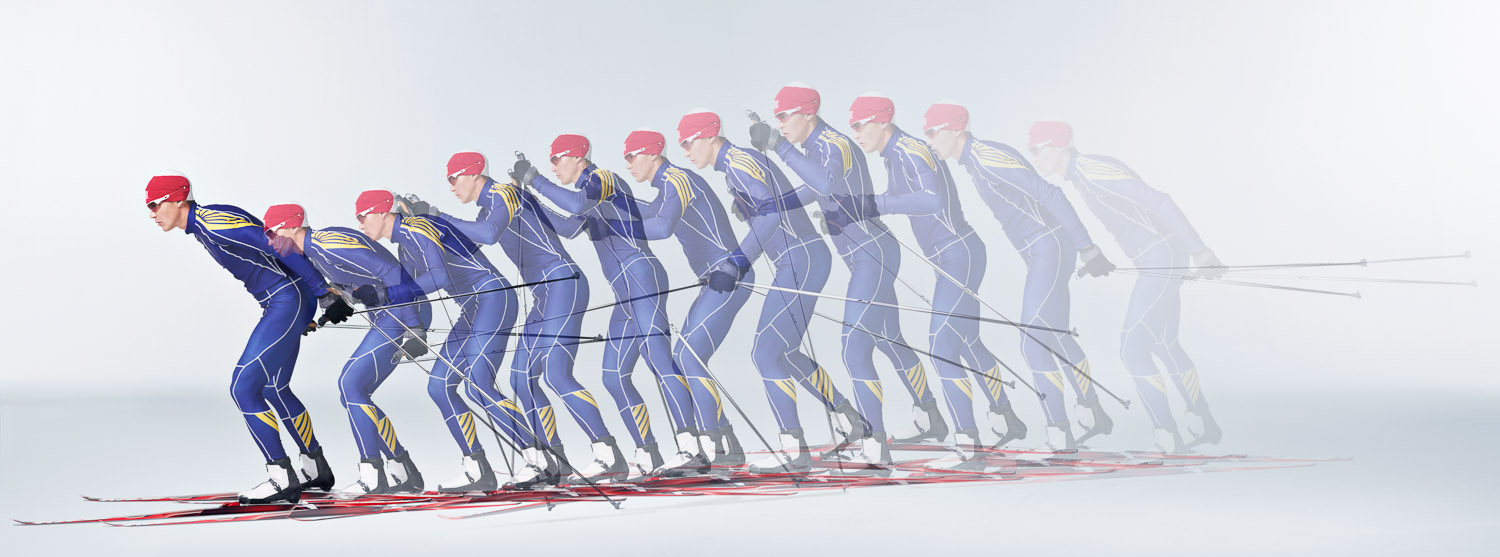
\includegraphics[width=0.8\textwidth]{Prototype/img/multiexposure}
  \caption{Athlete's movements captured in a multiple exposure image\cite{multiexposure}}
\label{fig:multiexposure}
\end{center}
\end{figure}

Up until this point the 3D graph would look as shown in figure \ref{fig:3DgraphDetail}. It visualizes up 2 variables over time. Even though the data is being visualized as an abstract triangulated body with hight and radius changes the sculpture could take advantage of the depth dimension not only to display volume but to steer the body also in this dimension. Through this realization, the 3D graph now can map 3 variables. To further enhance the aesthetic of the sculpture the concept of the athlete's snapshot in specific points of time was explored. For this a set of avatars performing different sports were developed. These avatars would intersect the graph body in specified intervals by the user. By adding different avatars performing a variety of sports users can chose the avatar that represents best the sport or activity the user did to generate the data. The sculpture could be expanded to support different decoration styles. For example apart from the triangulated look of the graph body, other visualization like a wire-frame option or a smoothed look could be offered. 
As shown in figure \ref{fig:3DgraphDetail}, the whole structure looks as if it would float in the air with the help of a support structure, which could be manufactured separately from transparent acrylic  so that they fade away centering the attention in the sculpture. This support structure would be inserted into a wooden or acrylic plate. The author explored the idea of engraving a summary of the data the sculpture represents. In this way users have both the abstract visualization and the actual data in the same place close enough to analyze. This might be useful while showing it to others, as it can help them better grasp how the sculpture was generated. By adding a plate to the sculpture we open a new set of configuration possibilities for users to edit in the configurator. 

The 3D graph embodies activity data through iconic and indexical representations. Indexical because as stated before, the concept emerged from an expanded line-chart an the graph body points to the path line-chart would have but abstracted and stylized and with the avatars in different positions point to movement in activity. The avatars are a strong icon of a human body in motion. The 3D graph shows a somewhat short metaphorical distance as the sculpture points strongly to the a line-chart metaphor used to embody the data. In the narrative formulation of the sculpture again the chart-graph resemblance and the plate tell the user this object is to be analyzed or at least admired as the plate does not allow grabbing the sculpture. Self reflection is highly encouraged as the metaphor motivates comparison of values over time. 

\begin{figure}[h]
\captionsetup{width=0.8\textwidth}
\begin{center}
  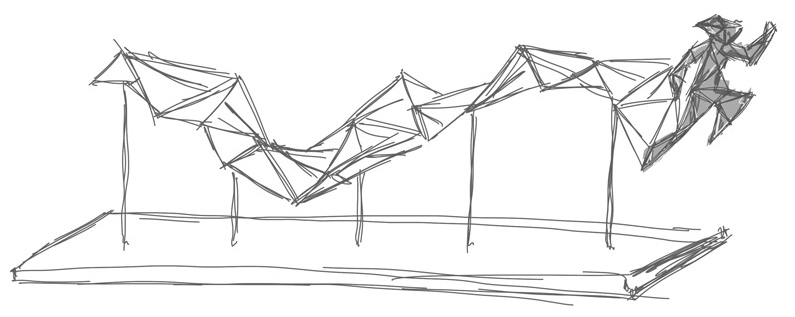
\includegraphics[width=0.8\textwidth]{Prototype/img/3DGraph_detail}
  \caption{3D Graph sketch}
\label{fig:3DgraphDetail}
\end{center}
\end{figure}

In summary the 3D Graph prototype is a highly aesthetic activity sculpture that is also functional as the both the sculpture and the data could be analyzed in the same object. The sculpture has a rather low capability of mapping several variables because of the constraints of the metaphor. This could be improved by adding more graph bodies representing each 3 variables over time. The 3D graph offers a wide range of configuration options that would make it a rather interesting object to customize in the configurator. The manufacturability of the sculpture is attainable but also complicated as the sculpture, the plate and the supporting elements have to be fabricated not to mention the engravings on the plate. 

\subsubsection{Activity Landscape}

\begin{figure}[h]
\centering
\begin{minipage}{.45\textwidth}
\centering
	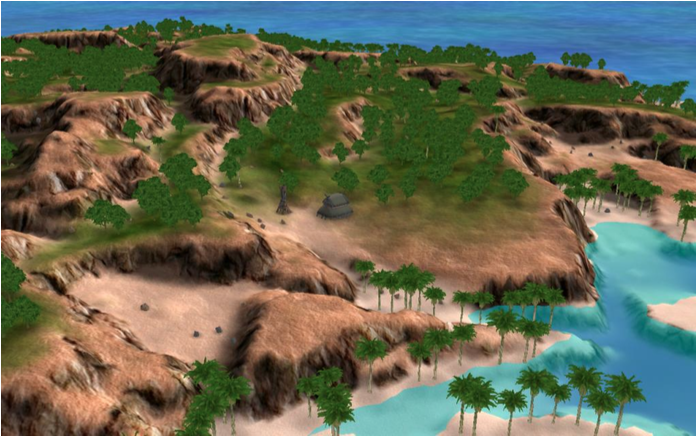
\includegraphics[width=\linewidth]{Prototype/img/terrain}
	\caption{Procedurally generated landscape \cite{olsen2004realtime}}
	\label{fig:proceduralterr}
\end{minipage}
\begin{minipage}{.45\textwidth}
\centering
  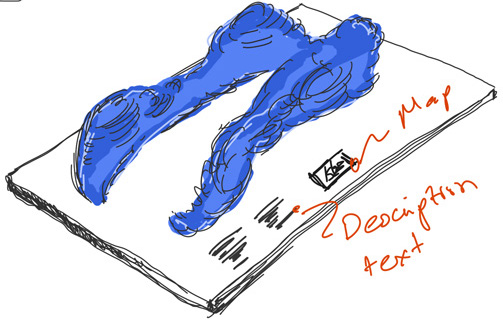
\includegraphics[width=0.88\linewidth]{Prototype/img/ActivityLandscape_detail}
  \caption{Activity Landscape sketch}
  \label{fig:activitylandscape}
\end{minipage}
\end{figure}


\subsubsection{Activity Flora}

\begin{figure}[h]
\captionsetup{width=0.9\textwidth}
\begin{center}
  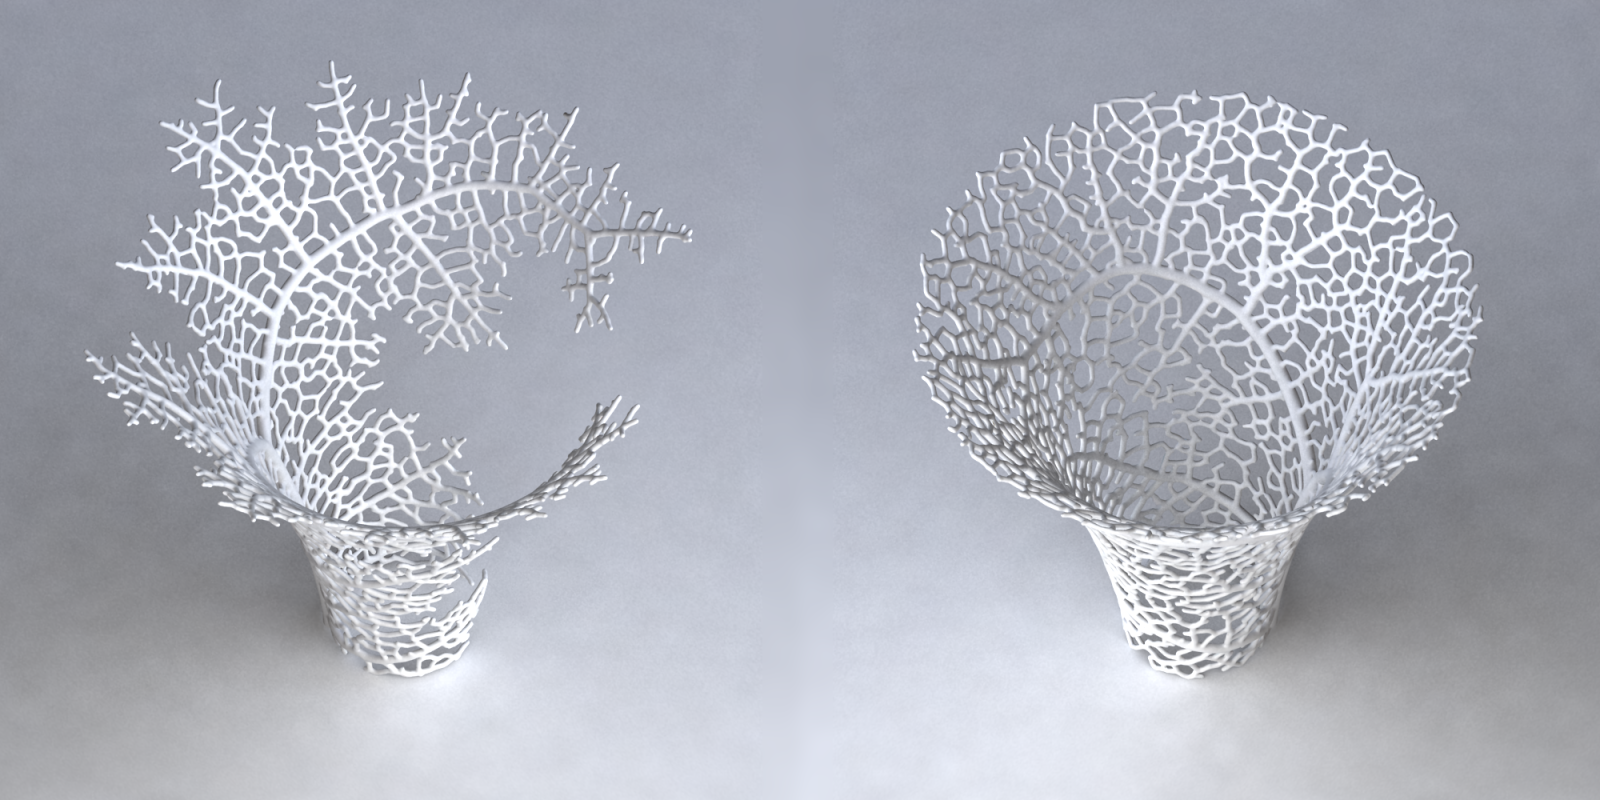
\includegraphics[width=0.9\textwidth]{Prototype/img/nervous}
  \caption{Sculptures made with generative algorithms based on hyphae growth as seen on leave and coral structures\cite{nervous}}
\label{fig:nervous}
\end{center}
\end{figure}

\begin{figure}[h]
\captionsetup{width=0.9\textwidth}
\begin{center}
  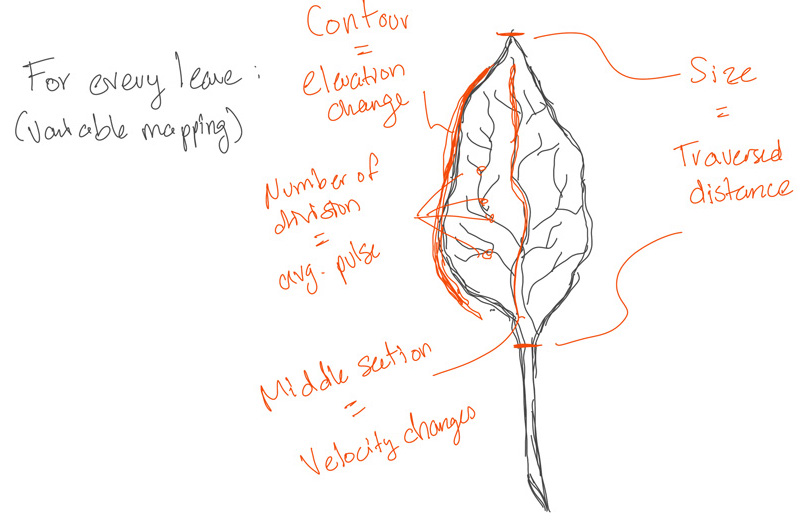
\includegraphics[width=0.7\textwidth]{Prototype/img/ActivityFlora_detail}
  \caption{Activity Flora sketch}
\label{fig:activityflora}
\end{center}
\end{figure}


\subsubsection{Activity Vase}

\begin{figure}[h]
\centering
\begin{minipage}{.45\textwidth}
\centering
	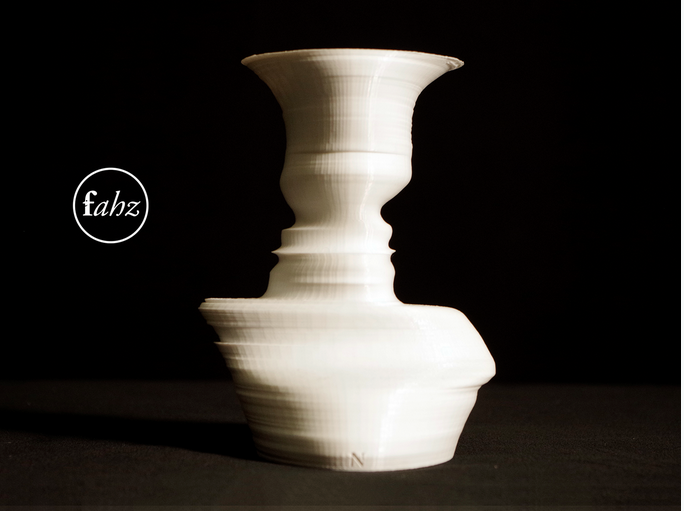
\includegraphics[width=\linewidth]{Prototype/img/fhaz}
	\caption{Fhaz: Procedurally generated vase based on facial profiles\cite{fahz}}
	\label{fig:fhaz}
\end{minipage}
\begin{minipage}{.45\textwidth}
\centering
  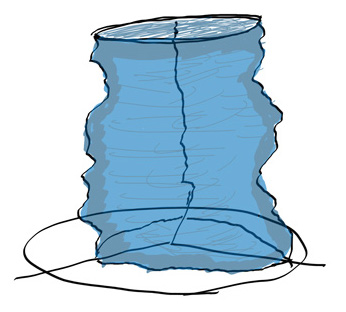
\includegraphics[width=0.75\linewidth]{Prototype/img/ActivityVase_detail}
  \caption{Activity Vase sketch}
  \label{fig:activityvase}
\end{minipage}
\end{figure}

\subsubsection{Prototype Validation}


\subsection{Configurator Design}
\cite{abbasi2012s}
\cite{Konstanzer20078609220}
\cite{rolland2012commerce}

\subsubsection{Ideation Process}


\begin{figure}[h]
\captionsetup{width=0.9\textwidth}
\begin{center}
  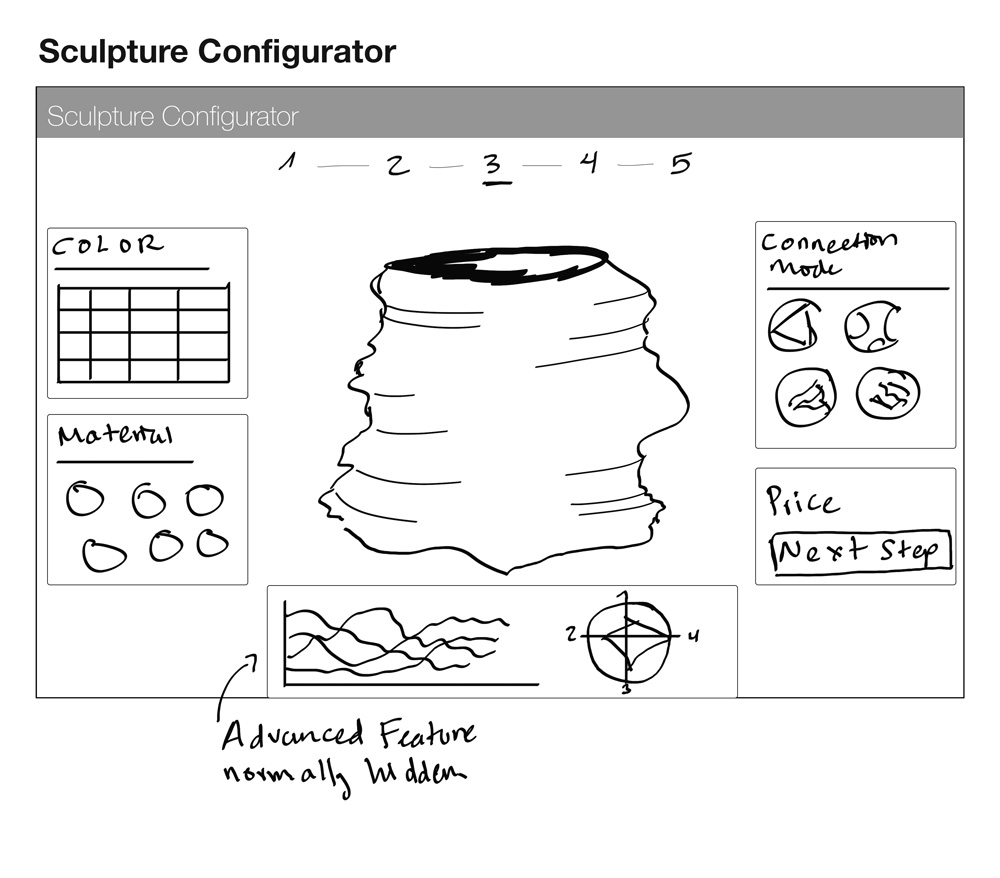
\includegraphics[width=0.6\textwidth]{Prototype/img/ui_proto1}
  \caption{Sketch of step based configurator prototype}
\label{fig:uiproto1}
\end{center}
\end{figure}

\begin{figure}[h]
\centering
\begin{minipage}{.45\textwidth}
\centering
  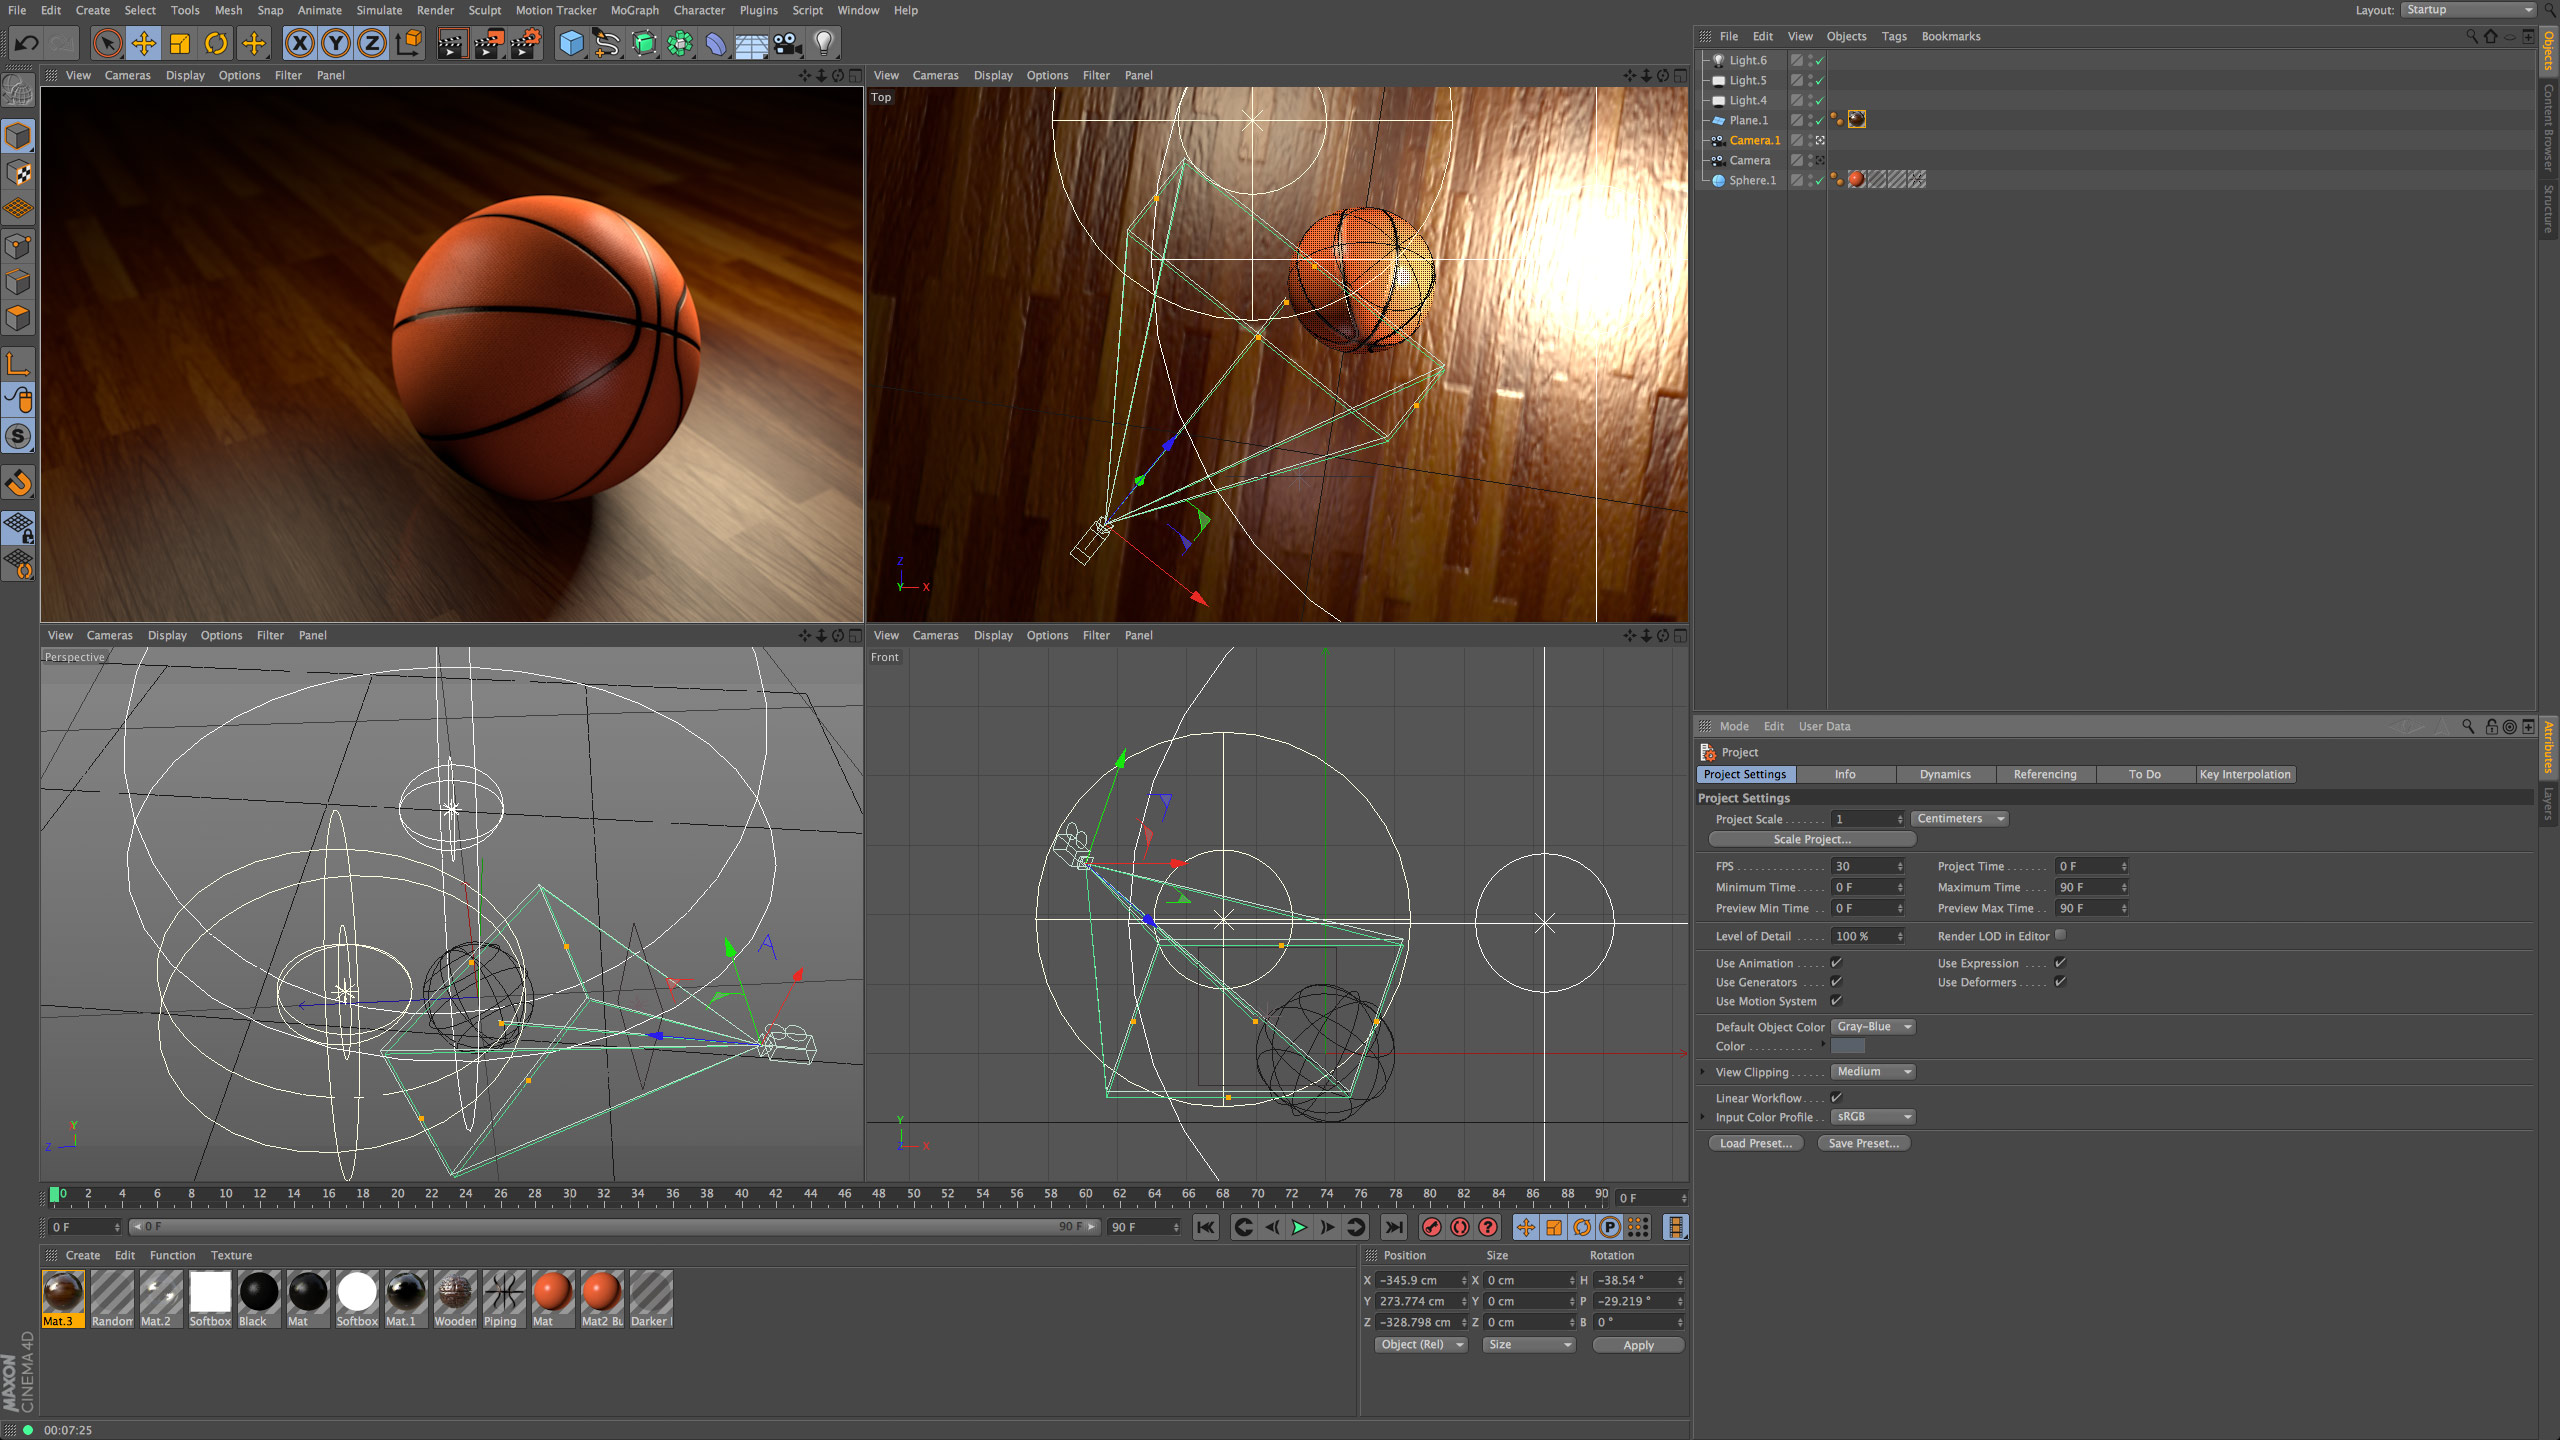
\includegraphics[width=\textwidth]{Prototype/img/cinema4d}
  \caption{3D modeling software Cinema 4D graphical user interface\cite{cinema4d}}
  \label{fig:cinema}
\end{minipage}
\begin{minipage}{.45\textwidth}
\centering
  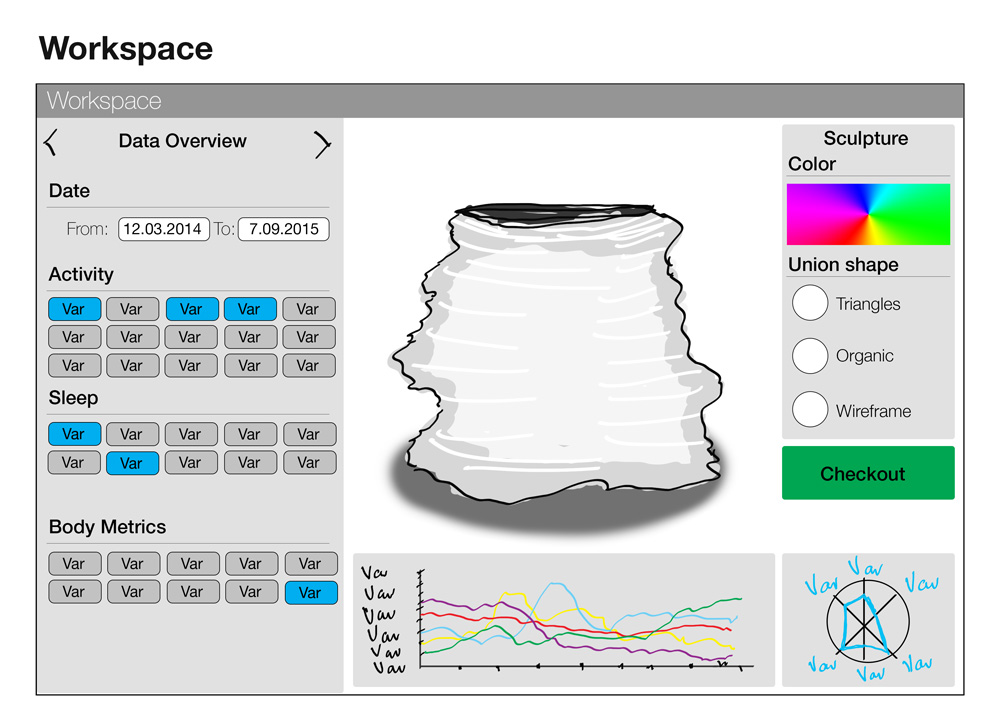
\includegraphics[width=\linewidth]{Prototype/img/ui_proto2}
  \caption{Sketch of 3D modeling software inspired configurator prototype}
  \label{fig:uiproto2}
\end{minipage}
\end{figure}

\begin{figure}[h]
\captionsetup{width=0.9\textwidth}
\begin{center}
  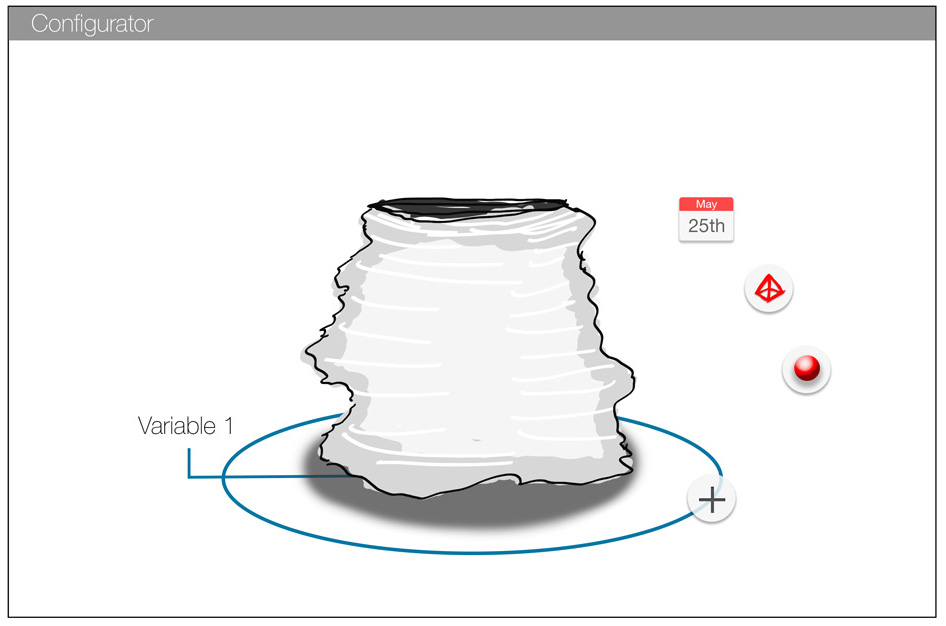
\includegraphics[width=0.6\textwidth]{Prototype/img/ui_proto3}
  \caption{Sketch of ``freestyle'' configurator prototype}
\label{fig:uiproto3}
\end{center}
\end{figure}

\subsubsection{Prototype Validation}

\end{document}